\documentclass{tufte-handout}

%\geometry{showframe}% for debugging purposes -- displays the margins

\usepackage{amsmath}

% Set up the images/graphics package
\usepackage{graphicx}
\setkeys{Gin}{width=\linewidth,totalheight=\textheight,keepaspectratio}
\graphicspath{{graphics/}}

% Correccion error: tightlist undefined sequence
\def\tightlist{}

% Correccion error: Argument of \MakeTextLowercase has an extra }
% Set up the spacing using fontspec features
\ifxetex
  \renewcommand\allcapsspacing[1]{{\addfontfeature{LetterSpace=15}#1}}
  \renewcommand\smallcapsspacing[1]{{\addfontfeature{LetterSpace=10}#1}}
\fi

\title{Harry Wong\thanks{Versión HV corta profesional}}
\author[Magister Ingeniería TI. Especializado en Arquitectura]{Magister
Ingeniería TI. Especializado en Arquitectura}
\date{24 Enero 2009}  % if the \date{} command is left out, the current date will be used

% The following package makes prettier tables.  We're all about the bling!
\usepackage{booktabs}

% The units package provides nice, non-stacked fractions and better spacing
% for units.
\usepackage{units}

% The fancyvrb package lets us customize the formatting of verbatim
% environments.  We use a slightly smaller font.
\usepackage{fancyvrb}
\fvset{fontsize=\normalsize}

% Small sections of multiple columns
\usepackage{multicol}

% Provides paragraphs of dummy text
\usepackage{lipsum}

% These commands are used to pretty-print LaTeX commands
\newcommand{\doccmd}[1]{\texttt{\textbackslash#1}}% command name -- adds backslash automatically
\newcommand{\docopt}[1]{\ensuremath{\langle}\textrm{\textit{#1}}\ensuremath{\rangle}}% optional command argument
\newcommand{\docarg}[1]{\textrm{\textit{#1}}}% (required) command argument
\newenvironment{docspec}{\begin{quote}\noindent}{\end{quote}}% command specification environment
\newcommand{\docenv}[1]{\textsf{#1}}% environment name
\newcommand{\docpkg}[1]{\texttt{#1}}% package name
\newcommand{\doccls}[1]{\texttt{#1}}% document class name
\newcommand{\docclsopt}[1]{\texttt{#1}}% document class option name

\begin{document}

\maketitle % this prints the handout title, author, and date



\begin{abstract}
\marginnote{
  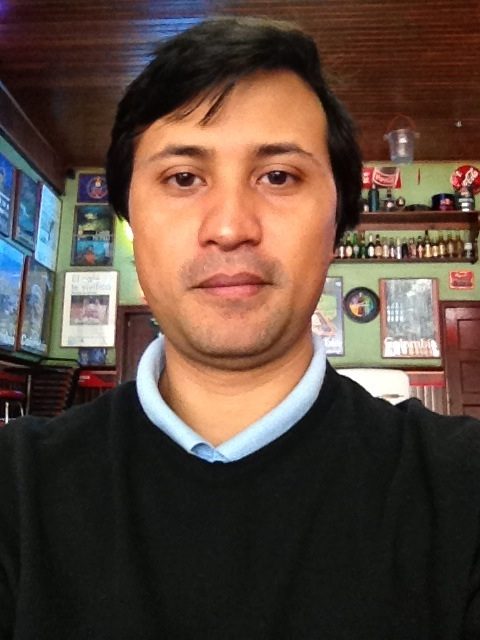
\includegraphics[width=\linewidth]{foto}
  Bogotá DC. Colombia

  K6 \# 48A 27

  Chapinero Alto

  T: 300 2818189

  hwong23@yahoo.com

  www.blazdesigns.com
}
    
\noindent Ing. de Sistemas. Arquitecto TI. Magister en Tecnologías de
Información para Negocio (MBIT, Uniandes). Especializado en Arquitectura
de Software Empresarial (AES, Javeriana). Certificado Arquitectura de
Software IASA CITAF. Certificado TOGAF 9.1 Nivel 1 y 2. Consultor
Tecnologías de Información y Transformación Negocio con Tecnología.
Consultor en mejoría de procesos de ingeniería. Consultor en
industrialización y construcción de software y sistemas de información.
Miembro de la Asociación de Arquitectos Empresariales, AEA. Miembro
Global IASA, Chapter Colombia. Miembro de ACIS (Asoc. Ing. de Sistemas).
Columnista independiente de Tecnología en LatinamericanPost.
\end{abstract}
  
%\printclassoptions
  
\section{Perfil}\label{sec:perfil}
En los más de 20 de mi trayecto de la ingeniería de sistemas he aplicado
los procesos de la ingeniería y tecnologías para abordar retos de
clientes de distintos sectores, público, privado, bancario, financiero,
seguros, fábricas de software, emprendimientos, entre otros. He
estudiado los procesos y los ciclos de la ingeniería de software, he
puesto en marcha tecnologías y paradigmas de desarrollo y de
arquitectura. Conozco el agilismo y el desarrollo continuo, práctica a
la que confiero confianza como transformadora extendida a la creación de
productos y negocios. He aprendido de la gestión del portafolio de
aplicaciones (Arquitectura Empresarial), y de la Dirección de TI. Los
posgrados, la Academia, los colegas ayudaron, y mucho; igual las áreas y
actividades en las que he trabajado, como el diseño y gestión de
servicios TI, Gobierno TI, planeación de TI, creación de oficinas de
arquitectura, analítica de datos, arquitectura de información,
integración de aplicaciones de empresas, análisis de los procesos de
negocio, y una de mis preferidas, la ingeniería de modelos y la
automatización del software, ahora impulsada la inteligencia artificial.
Lo anterior hace que me oriente a la colaboración: una arquitectura no
se hace en aislamiento. La comunicación y la colaboración son
preponderante en la relación con las unidades de negocio, gerentes de
proyectos, operación, jefes de infraestructura, dueños de procesos,
productos, expertos de negocio, líderes funcionales, y por supuesto, con
mis colegas ingenieros. La tecnología, la ingeniería y la arquitectura
son todas una pasión, y mi trabajo. Procuro posicionarlas y tender
diálogos con otras disciplinas, como la economía y los negocios.
Sostengo que el software, distinto a otras construcciones, es moldeable,
incremental, de naturaleza cambiante. Sé también que hay que conjugar
los intereses con los resultados, incluso por fuera de los métodos
formales, con el fin de entregar logros a beneficiarios, interesados,
dueños de negocio, interventores, auditores; lo mismo a colegas, con
quienes disfruto argumentar. Por último, la escritura se ha convertido
en un ejercicio del que disfruto y, que no debe ser sorpresa,
complementa a la perfección mi trabajo: la documentación técnica. Desde
el 2018 escribo en sitios de opinión y soy columnista independiente de
tecnología en LatinamericanPost.

\section{Formación}\label{sec:formacion}
\marginnote{
  En los más de 20 de mi trayecto de la ingeniería de sistemas he
  aplicado los procesos de la ingeniería y tecnologías para abordar
  retos de clientes de distintos sectores, público, privado, bancario,
  financiero, seguros, fábricas de software, emprendimientos, entre
  otros. He estudiado los procesos y los ciclos de la ingeniería de
  software, he puesto en marcha tecnologías y paradigmas de desarrollo y
  de arquitectura. Conozco el agilismo y el desarrollo continuo,
  práctica a la que confiero confianza como transformadora extendida a
  la creación de productos y negocios. He aprendido de la gestión del
  portafolio de aplicaciones (Arquitectura Empresarial), y de la
  Dirección de TI. Los posgrados, la Academia, los colegas ayudaron, y
  mucho; igual las áreas y actividades en las que he trabajado, como el
  diseño y gestión de servicios TI, Gobierno TI, planeación de TI,
  creación de oficinas de arquitectura, analítica de datos, arquitectura
  de información, integración de aplicaciones de empresas, análisis de
  los procesos de negocio, y una de mis preferidas, la ingeniería de
  modelos y la automatización del software, ahora impulsada la
  inteligencia artificial. Lo anterior hace que me oriente a la
  colaboración: una arquitectura no se hace en aislamiento. La
  comunicación y la colaboración son preponderante en la relación con
  las unidades de negocio, gerentes de proyectos, operación, jefes de
  infraestructura, dueños de procesos, productos, expertos de negocio,
  líderes funcionales, y por supuesto, con mis colegas ingenieros. La
  tecnología, la ingeniería y la arquitectura son todas una pasión, y mi
  trabajo. Procuro posicionarlas y tender diálogos con otras
  disciplinas, como la economía y los negocios. Sostengo que el
  software, distinto a otras construcciones, es moldeable, incremental,
  de naturaleza cambiante. Sé también que hay que conjugar los intereses
  con los resultados, incluso por fuera de los métodos formales, con el
  fin de entregar logros a beneficiarios, interesados, dueños de
  negocio, interventores, auditores; lo mismo a colegas, con quienes
  disfruto argumentar. Por último, la escritura se ha convertido en un
  ejercicio del que disfruto y, que no debe ser sorpresa, complementa a
  la perfección mi trabajo: la documentación técnica. Desde el 2018
  escribo en sitios de opinión y soy columnista independiente de
  tecnología en LatinamericanPost.
}
\begin{itemize}
\tightlist
\item
  Diplomado de Analítica de Datos (2022), Pontificia Universidad
  Javeriana. Bogotá.
\item
  Analítica de Datos y Automatización de Procesos en Power BI y
  Automate. (2021). Educación Continua de la Pontificia Universidad
  Javeriana. Bogotá
\item
  Práctica de Aprendizaje Reforzado. Ciclo de Inteligencia Artificial.
  (2021). Universidad de los Andes. Bogotá
\item
  Gestión de Contenidos Digitales. (2020). Educación Continua de la
  Pontificia Universidad Javeriana. Bogotá.
\item
  Diseño de Información. (2019). Centro de Estudios en Periodismo
  (CEPER). Universidad de los Andes. Bogotá.
\item
  Diplomado de Gestión y Diseño de Productos Digitales. (2019).
  Universidad Nacional. Bogotá.
\item
  Periodismo Escrito para no Periodistas. (2018). Universidad de los
  Andes. Bogotá\textless{}
\item
  Maestría en Tecnologías de Información para Negocio (2015).
  Universidad de los Andes. Bogotá.
\item
  Especialización de Arquitectura Empresarial de Software (2012),
  Pontificia Universidad Javeriana. Bogotá.
\item
  IASA Core Architecture Foundation Certification. (2013). Universidad
  de los Andes; Colombia: Bogotá.
\item
  TOGAF 9 Certified, Global AEA. (2015). Colombia: Bogotá.
\item
  TOGAF 9 Foundation, Global AEA; (2015). Colombia: Bogotá.
\item
  Arquitectura TI Colombia, Global AEA; Bogotá - Colombia, 2015
\item
  SOA Architect Certification Course, it-education, SOA School; Bogotá -
  Colombia, 2014.
\item
  Metodología ICES, Iniciativa de Ciudades Emergentes y Sostenibles,
  2016, BID - Edx.
\item
  Implementing Data Warehouse / MSSQL Server 2014, Intelligent Training
  - Colombia, 2016
\item
  Desarrollo y Administración Oracle 10g, Universidad Católica Santiago
  de Guayaquil, Guayaquil - Ecuador, Ing. Sistemas Computacionales, 2010
\item
  Graduado de Ingeniería en Sistemas de Información (2000), Universidad
  Católica Santiago de Guayaquil
\end{itemize}

\section{Experiencias}\label{sec:experiencias}
\begin{itemize}
\tightlist
\item
  Consultor externo de proyectos de arquitectura, ingeniería y
  tecnología para Estefanini, Colombia.
\item
  Contratista para el BID y el Ministerio del Trabajo de Colombia, en el
  cargo de consultor arquitecto de software para proyectos de diseño e
  implementación de sistemas de información para el Programa de
  Fortalecimiento al Empleo y del Mercado Laboral
\item
  20+ años de experiencia en el campo de TI, tecnologías probadas y
  nuevas, ingeniería de procesos y de sistemas, proyectos de TI
\item
  Diseño y construcción de integración de arquitecturas reactivas,
  asíncronas, orientadas a eventos
\item
  Diseño e integración de sistemas distribuidos, de apoyo a procesos de
  negocio, basados en arquitectura de componentes, servicios modulares,
  microservicios y SOA
\item
  Experiencia en administración de tecnologías para proyectos de
  ciudades inteligentes
\item
  Experiencia en administración de tecnologías para proyectos de gestión
  documental
\item
  Conocimiento en manejo de operación de TI con orientación a Servicios
  de TI (basados en ITIL)
\item
  Experiencia en Tecnología de Modelos (Model Driven Engineering, MDE)
  para especificación, diseño y automatización de construcción y
  mantenimiento de sistemas de información y software
\item
  Aplicación y selección de métodos y herramientas de ALM (ciclo de vida
  de aplicaciones de software) con énfasis en diseño
\item
  Aplicación de principios de arquitectura de software, diseño de
  sistemas: patrones convencionales y emergentes y teoría de sistemas de
  información
\item
  Experiencia en métodos de estimación de proyectos de tecnología,
  software, costos, calidad, relación con la Arquitectura de Software y
  de Negocio
\item
  Experiencia en implementación de Sistemas de Información en
  combinación de Agilismo y gerencia de proyectos, PMI (Project
  Management Institute)
\item
  Trayectoria en manejo y mejora del rendimiento de equipos de
  Ingeniería bajo métodos de industrialización y automatización para la
  construcción de software
\item
  Especialista en soluciones de negocio distribuidas y orientadas a
  sistemas de misión crítica como banca en línea, canales electrónicos,
  y automatización de procesos
\item
  Aplicación de métodos para generación y gestión de cambios
  tecnológicos de alto-impacto para la empresa
\item
  Conocimiento y aplicación de lenguajes específicos de dominio (DSL)
  para acelerar la comunicación y la producción de artefactos para las
  áreas de negocio, interesados, administradores, arquitectos y otros
  ingenieros
\end{itemize}


\section{Page Layout}\label{sec:page-layout}
\subsection{Headings}\label{sec:headings}
This style provides \textsc{a}- and \textsc{b}-heads (that is, 
\Verb|\section| and \Verb|\subsection|), demonstrated above.

The Tufte-\LaTeX\ classes will emit an error if you try to use 
\linebreak\Verb|\subsubsection| and smaller headings.

% let's start a new thought -- a new section
\newthought{In his later books}, cite Cabezon2024 Tufte
starts each section with a bit of vertical space, a non-indented paragraph,
and sets the first few words of the sentence in \textsc{small caps}.  To
accomplish this using this style, use the \Verb|\newthought| command:  
\begin{docspec}
  \doccmd{newthought\{In his later books\}, Tufte starts\ldots}
\end{docspec}

\subsection{Sidenotes}\label{sec:sidenotes}
One of the most prominent and distinctive features of this style is the
extensive use of sidenotes.  There is a wide margin to provide ample room
for sidenotes and small figures. Any \Verb|\footnote|s will automatically
be converted to sidenotes.
\footnote{
   This is a sidenote that was entered
  using the \texttt{\textbackslash footnote} command.
  }
If you'd like to place ancillary
information in the margin without the sidenote mark (the superscript
number), you can use the \Verb|\marginnote| command.\marginnote{This is a
margin note.  Notice that there isn't a number preceding the note, and
there is no number in the main text where this note was written.}

The specification of the \Verb|\sidenote| command is:
\begin{docspec}
  \doccmd{sidenote[\docopt{number}][\docopt{offset}]\{\docarg{Sidenote text.}\}}
\end{docspec}

Both the \docopt{number} and \docopt{offset} arguments are optional.  If you
provide a \docopt{number} argument, then that number will be used as the
sidenote number.  It will change of the number of the current sidenote only and
will not affect the numbering sequence of subsequent sidenotes.

Sometimes a sidenote may run over the top of other text or graphics in the
margin space.  If this happens, you can adjust the vertical position of the
sidenote by providing a dimension in the \docopt{offset} argument.  Some
examples of valid dimensions are:
\begin{docspec}
  \ttfamily 1.0in \qquad 2.54cm \qquad 254mm \qquad 6\Verb|\baselineskip|
\end{docspec}
If the dimension is positive it will push the sidenote down the page; if the
dimension is negative, it will move the sidenote up the page.

While both the \docopt{number} and \docopt{offset} arguments are optional, they
must be provided in order.  To adjust the vertical position of the sidenote
while leaving the sidenote number alone, use the following syntax:
\begin{docspec}
  \doccmd{sidenote[][\docopt{offset}]\{\docarg{Sidenote text.}\}}
\end{docspec}
The empty brackets tell the \Verb|\sidenote| command to use the default
sidenote number.

If you \emph{only} want to change the sidenote number, however, you may
completely omit the \docopt{offset} argument:
\begin{docspec}
  \doccmd{sidenote[\docopt{number}]\{\docarg{Sidenote text.}\}}
\end{docspec}

The \Verb|\marginnote| command has a similar \docarg{offset} argument:
\begin{docspec}
  \doccmd{marginnote[\docopt{offset}]\{\docarg{Margin note text.}\}}
\end{docspec}

\subsection{References}
References are placed alongside their citations as sidenotes,
as well.  This can be accomplished using the normal \Verb|\cite|
command.\sidenote{The first paragraph of this document includes a citation.}

The complete list of references may also be printed automatically by using
the \Verb|\bibliography| command.  (See the end of this document for an
example.)  If you do not want to print a bibliography at the end of your
document, use the \Verb|\nobibliography| command in its place.  

To enter multiple citations at one location,cite{Tufte2006,Tufte1990} you can
provide a list of keys separated by commas and the same optional vertical
offset argument: \Verb|\cite{Tufte2006,Tufte1990}|.  
\begin{docspec}
  \doccmd{cite[\docopt{offset}]\{\docarg{bibkey1,bibkey2,\ldots}\}}
\end{docspec}

\section{Figures and Tables}\label{sec:figures-and-tables}
Images and graphics play an integral role in Tufte's work.
In addition to the standard \docenv{figure} and \docenv{tabular} environments,
this style provides special figure and table environments for full-width
floats.

Full page--width figures and tables may be placed in \docenv{figure*} or
\docenv{table*} environments.  To place figures or tables in the margin,
use the \docenv{marginfigure} or \docenv{margintable} environments as follows
(see figure~\ref{fig:marginfig}):

\begin{marginfigure}%
  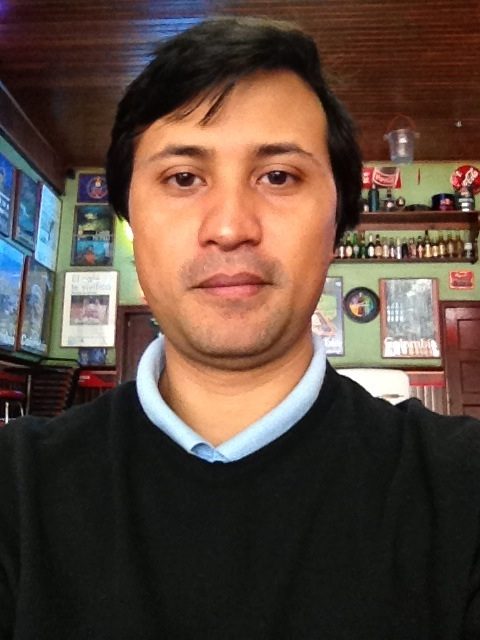
\includegraphics[width=\linewidth]{foto}
  % \÷caption{
    \noindent{Bogotá DC. Colombia

K6 \# 48A 27

Chapinero Alto

T: 300 2818189

hwong23@yahoo.com

www.blazdesigns.com}
  % }
  \label{fig:marginfig}
\end{marginfigure}

\begin{Verbatim}
\begin{marginfigure}
  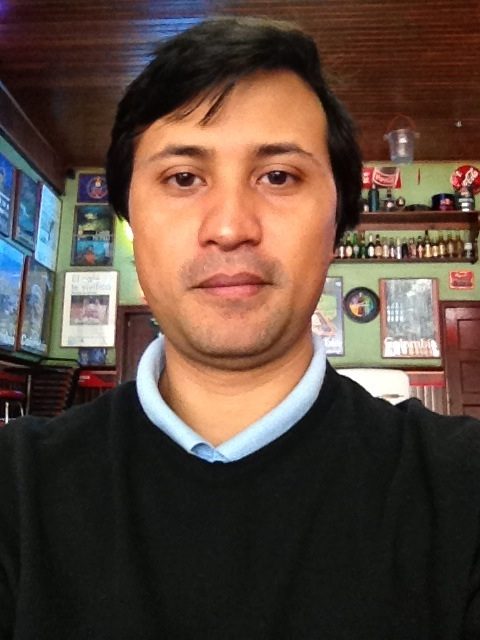
\includegraphics{foto}
  \caption{This is a margin figure.}
\end{marginfigure}
\end{Verbatim}

The \docenv{marginfigure} and \docenv{margintable} environments accept an optional 
parameter \docopt{offset} that adjusts the vertical position of the figure or table.  
See the ``\nameref{sec:sidenotes}'' section above for examples.  The specifications are:
\begin{docspec}
  \doccmd{begin\{marginfigure\}[\docopt{offset}]}\\
  \qquad\ldots\\
  \doccmd{end\{marginfigure\}}\\
  \mbox{}\\
  \doccmd{begin\{margintable\}[\docopt{offset}]}\\
  \qquad\ldots\\
  \doccmd{end\{margintable\}}\\
\end{docspec}

Figure~\ref{fig:fullfig} is an example of the \Verb|figure*|
environment and figure~\ref{fig:textfig} is an example of the normal
\Verb|figure| environment.

\begin{figure*}[h]
  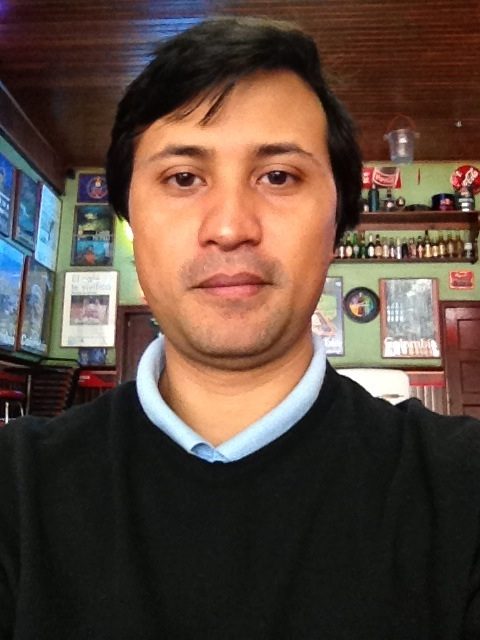
\includegraphics[width=\linewidth]{foto.png}%
  \caption{This graph shows y = sin x from about x = [-10, 10].
  \emph{Notice that this figure takes up the full page width.}}%
  \label{fig:fullfig}%
\end{figure*}

\begin{figure}
  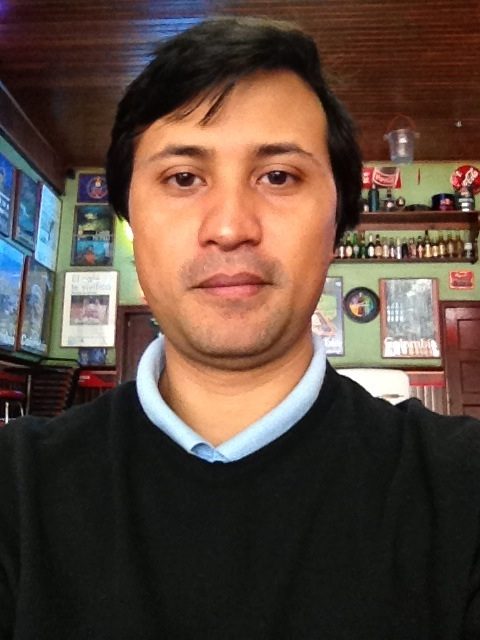
\includegraphics{foto.png}
%  \checkparity This is an \pageparity\ page.%
  \caption{Hilbert curves of various degrees .
  \emph{Notice that this figure only takes up the main textblock width.}}
  \label{fig:textfig}
  %\zsavepos{pos:textfig}
  \setfloatalignment{b}
\end{figure}

Table~\ref{tab:normaltab} shows table created with the \docpkg{booktabs}
package.  Notice the lack of vertical rules---they serve only to clutter
the table's data.

\begin{table}[ht]
  \centering
  \fontfamily{ppl}\selectfont
  \begin{tabular}{ll}
    \toprule
    Margin & Length \\
    \midrule
    Paper width & \unit[8\nicefrac{1}{2}]{inches} \\
    Paper height & \unit[11]{inches} \\
    Textblock width & \unit[6\nicefrac{1}{2}]{inches} \\
    Textblock/sidenote gutter & \unit[\nicefrac{3}{8}]{inches} \\
    Sidenote width & \unit[2]{inches} \\
    \bottomrule
  \end{tabular}
  \caption{Here are the dimensions of the various margins used in the Tufte-handout class.}
  \label{tab:normaltab}
  %\zsavepos{pos:normaltab}
\end{table}

\section{Full-width text blocks}

In addition to the new float types, there is a \docenv{fullwidth}
environment that stretches across the main text block and the sidenotes
area.

\begin{Verbatim}
\begin{fullwidth}
Lorem ipsum dolor sit amet...
\end{fullwidth}
\end{Verbatim}

\begin{fullwidth}
\small\itshape\lipsum[1]
\end{fullwidth}

\section{Typography}\label{sec:typography}

\subsection{Typefaces}\label{sec:typefaces}
If the Palatino, \textsf{Helvetica}, and \texttt{Bera Mono} typefaces are installed, this style
will use them automatically.  Otherwise, we'll fall back on the Computer Modern
typefaces.

When setting strings of \allcaps{ALL CAPS} or \smallcaps{small caps}, the
letter\-spacing---that is, the spacing between the letters---should be
increased slightly.cite Bringhurst2005  The \Verb|\allcaps| command has proper letterspacing for
strings of \allcaps{FULL CAPITAL LETTERS}, and the \Verb|\smallcaps| command
has letterspacing for \smallcaps{small capital letters}. These commands
will also automatically convert the case of the text to upper- or
lowercase, respectively.

The \Verb|\textsc| command has also been redefined to include
letterspacing.  The case of the \Verb|\textsc| argument is left as is,
however.  This allows one to use both uppercase and lowercase letters:
\textsc{The Initial Letters Of The Words In This Sentence Are Capitalized.}

\subsection{Letterspacing}\label{sec:letterspacing}
This document class includes two new commands and some improvements on
existing commands for letterspacing.

The \Verb|\textsc| command has also been redefined to include
letterspacing.  The case of the \Verb|\textsc| argument is left as is,
however.  This allows one to use both uppercase and lowercase letters:
\textsc{The Initial Letters Of The Words In This Sentence Are Capitalized.}

\section{Installation}\label{sec:installation}
To install the Tufte-\LaTeX\ classes, simply drop the
following files into the same directory as your \texttt{.tex}
file:
\begin{quote}
  \ttfamily
  tufte-common.def\\
  tufte-handout.cls\\
  tufte-book.cls
\end{quote}

% TODO add instructions for installing it globally



\section{More Documentation}\label{sec:more-doc}
For more documentation on the Tufte-\LaTeX{} document classes (including commands not
mentioned in this handout), please see the sample book.

\section{Support}\label{sec:support}

\bibliography{sample-handout}
\bibliographystyle{plainnat}



\end{document}
